\let\negmedspace\undefined
\let\negthickspace\undefined
\documentclass[journal]{IEEEtran}
\usepackage[a5paper, margin=10mm, onecolumn]{geometry}
%\usepackage{lmodern} % Ensure lmodern is loaded for pdflatex
\usepackage{tfrupee} % Include tfrupee package

\setlength{\headheight}{1cm} % Set the height of the header box
\setlength{\headsep}{0mm}     % Set the distance between the header box and the top of the text

\usepackage{gvv-book}
\usepackage{gvv}
\usepackage{cite}
\usepackage{amsmath,amssymb,amsfonts,amsthm}
\usepackage{algorithmic}
\usepackage{graphicx}
\usepackage{textcomp}
\usepackage{xcolor}
\usepackage{txfonts}
\usepackage{listings}
\usepackage{enumitem}
\usepackage{mathtools}
\usepackage{gensymb}
\usepackage{comment}
\usepackage[breaklinks=true]{hyperref}
\usepackage{tkz-euclide} 
\usepackage{listings}
% \usepackage{gvv}                                        
\def\inputGnumericTable{}                   
\usepackage[latin1]{inputenc}                                
\usepackage{color}                                            
\usepackage{array}                                                 
\usepackage{longtable}                                       
\usepackage{calc}                                                 
\usepackage{multirow}                                         
\usepackage{hhline}                                           
\usepackage{ifthen}                                           
\usepackage{lscape}
\usepackage{circuitikz}
\usepackage{multicol}


\renewcommand{\thefigure}{\theenumi}
\renewcommand{\thetable}{\theenumi}
\setlength{\intextsep}{10pt} % Space between text and floats


\numberwithin{equation}{enumi}
\numberwithin{figure}{enumi}
\renewcommand{\thetable}{\theenumi}


% Marks the beginning of the document
\begin{document}
\bibliographystyle{IEEEtran}
\vspace{3cm}

\title{GATE 2014}
\author{EY: Ecology \& Evolution}
\maketitle

% (add your content here)
\noindent \textbf{General Aptitude}
\newline
\newline
\noindent \textbf{Q. 1 -- Q. 5} carry one mark each.

\begin{enumerate}
    \item A student is required to demonstrate a high level of comprehension of the subject, especially in the social sciences. \newline The word closest in meaning to comprehension is

    \begin{multicols}{4}
    \begin{enumerate}
        \item understanding
        \item meaning
        \item concentration
        \item stability
    \end{enumerate}
    \end{multicols}
    \hfill{$\brak{ GATE\ EY\ 2014}$}
    \bigskip
    
    \item Choose the most appropriate word from the options given below to complete the following sentence. \newline One of his biggest \rule{3cm}{0.15mm} was his ability to forgive.
    \begin{multicols}{4}
    \begin{enumerate}
        \item vice
        \item virtues
        \item choices
        \item strength
    \end{enumerate}
    \end{multicols}
    \hfill{$\brak{ GATE\ EY\ 2014}$}
    \bigskip

    \item Rajan was not happy that Sajan decided to do the project on his own. On observing his unhappiness, Sajan explained to Rajan that he preferred to work independently. \newline Which one of the statements below is logically valid and can be inferred from the above sentences?
    \begin{enumerate}
        \item Rajan has decided to work only in a group.
        \item Rajan and Sajan were formed into a group against their wishes.
        \item Sajan had decided to give in to Rajan's request to work with him.
        \item Rajan had believed that Sajan and he would be working together.
    \end{enumerate}
    \hfill{$\brak{ GATE\ EY\ 2014}$}
    \bigskip

    \item If $y=5x^{2}+3$, then the tangent at $x=0, y=3$
    \begin{multicols}{2}
    \begin{enumerate}
        \item passes through $x=0, y=0$
        \item has a slope of $+1$
        \item is parallel to the x-axis
        \item has a slope of $-1$
    \end{enumerate}
    \end{multicols}
    \hfill{$\brak{ GATE\ EY\ 2014}$}
    \bigskip

    \item A foundry has a fixed daily cost of Rs $50,000$ whenever it operates and a variable cost of Rs $800$Q, where Q is the daily production in tonnes. What is the cost of production in Rs per tonne for a daily production of $100$ tonnes? \rule{3cm}{0.15mm}

    \hfill{$\brak{ GATE\ EY\ 2014}$}
    \bigskip
\end{enumerate}

\noindent \textbf{Q. 6 -- Q. 10} carry two marks each.

\begin{enumerate}
\setcounter{enumi}{5}
    \item Find the odd one in the following group: ALRVX, EPVZB, ITZDF, OYEIK
    \begin{multicols}{4}
    \begin{enumerate}
        \item ALRVX
        \item EPVZB
        \item ITZDF
        \item OYEIK
    \end{enumerate}
    \end{multicols}
    \hfill{$\brak{ GATE\ EY\ 2014}$}
    \bigskip

    \item Anuj, Bhola, Chandan, Dilip, Eswar and Faisal live on different floors in a six-storeyed building (the ground floor is numbered $1$, the floor above it $2$, and so on). Anuj lives on an even-numbered floor. Bhola does not live on an odd numbered floor. Chandan does not live on any of the floors below Faisal's floor. Dilip does not live on floor number $2$. Eswar does not live on a floor immediately above or immediately below Bhola. Faisal lives three floors above Dilip. Which of the following floor-person combinations is correct?
    \newline
    \begin{figure}[H]
    \centering
    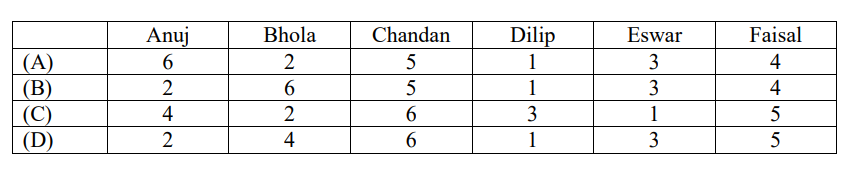
\includegraphics[width=0.8\columnwidth]{figs/1.png}
    \caption{}
    \label{fig:1}
   \end{figure}
    \hfill{$\brak{ GATE\ EY\ 2014}$}
    \bigskip

    \item The smallest angle of a triangle is equal to two thirds of the smallest angle of a quadrilateral. The ratio between the angles of the quadrilateral is $3:4:5:6$. The largest angle of the triangle is twice its smallest angle. What is the sum, in degrees, of the second largest angle of the triangle and the largest angle of the quadrilateral? \rule{3cm}{0.15mm}
    \hfill{$\brak{ GATE\ EY\ 2014}$}
    \bigskip

    \item One percent of the people of country X are taller than $6$ ft. Two percent of the people of country Y are taller than $6$ ft. There are thrice as many people in country X as in country Y. Taking both countries together, what is the percentage of people taller than $6$ ft?
    \begin{multicols}{4}
    \begin{enumerate}
        \item $3.0$
        \item $2.5$
        \item $1.5$
        \item $1.25$
    \end{enumerate}
    \end{multicols}
    \hfill{$\brak{ GATE\ EY\ 2014}$}
    \bigskip

    \item The monthly rainfall chart based on $50$ years of rainfall in Agra is shown in the following figure. Which of the following are true? (k percentile is the value such that k percent of the data fall below that value)
    \begin{figure}[H]
    \centering
    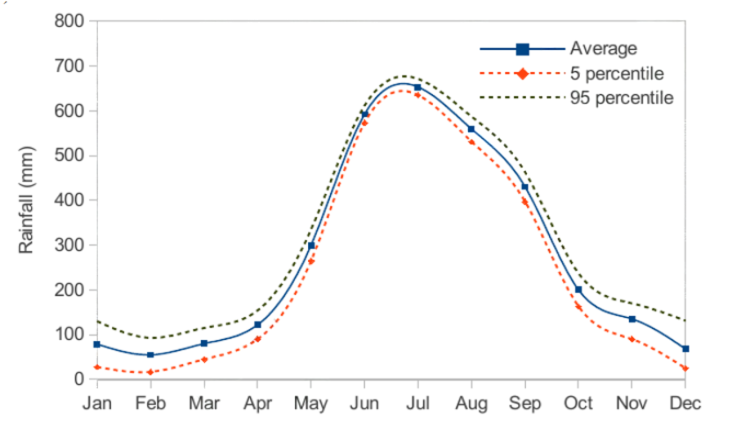
\includegraphics[width=0.8\columnwidth]{figs/2.png}
    \caption{}
    \label{fig:2}
   \end{figure}
    \begin{enumerate}
        \item $\brak{(i)}$ On average, it rains more in July than in December
        \item $\brak{(ii)}$ Every year, the amount of rainfall in August is more than that in January
        \item $\brak{(iii)}$ July rainfall can be estimated with better confidence than February rainfall
        \item $\brak{(iv)}$ In August, there is at least $500$ mm of rainfall
    \end{enumerate}
    \begin{multicols}{2}
    \begin{enumerate}
        \item $\brak{i}$ and $\brak{ii}$
        \item $\brak{i}$ and $\brak{i}$
        \item $\brak{iii}$ and $\brak{iv}$
        \item $\brak{(iii)}$ and $\brak{iv}$
    \end{enumerate}
    \end{multicols}
    \hfill{$\brak{ GATE\ EY\ 2014}$}
\end{enumerate}

\newpage
\noindent \textbf{ECOLOGY \& EVOLUTION - EY}
\newline
\newline
\noindent \textbf{Q. 1 -- Q. 25} carry one mark each.
\begin{enumerate}

    \item Darwin's ideas on evolution by natural selection were influenced by
    \begin{multicols}{2}
    \begin{enumerate}
        \item Lyell and Malthus
        \item Watson and Crick
        \item Meselson and Stahl
        \item Miller and Urey
    \end{enumerate}
    \end{multicols}
    \hfill{$\brak{ GATE\ EY\ 2014}$}
    \bigskip
    
    \item Which of the following statements about the evolution of humans is believed to be TRUE?
    \begin{enumerate}
        \item Modern day humans evolved from Neanderthals
        \item Modern day humans and Neanderthals share a recent common ancestor
        \item Modern day humans and Neanderthals both evolved from chimpanzees
        \item Modern day humans evolved from chimpanzees
    \end{enumerate}
    \hfill{$\brak{ GATE\ EY\ 2014}$}
    \bigskip

    \item On average, which ecosystem has the LOWEST net primary productivity per unit area?
    \begin{multicols}{2}
    \begin{enumerate}
        \item An open ocean
        \item A coral reef
        \item An estuary
        \item A fresh water lake
    \end{enumerate}
    \end{multicols}
    \hfill{$\brak{ GATE\ EY\ 2014}$}
    \bigskip

    \item A researcher measures the height of $100$ trees of a species. The mean of these observations is $50$ and the variance is $16$. The standard error of the mean calculated from these observations is \rule{3cm}{0.15mm}
    \hfill{$\brak{ GATE\ EY\ 2014}$}
    \bigskip
    
    \item A researcher tested for the presence of parasitic infection in $100$ male and $100$ female deer. Forty males and $30$ females were found to be infected. To test if males are significantly more susceptible to infection than females, which of the following is an appropriate statistical test?
    \begin{multicols}{2}
    \begin{enumerate}
        \item Student's t-test
        \item Mann-Whitney U test
        \item Chi-square test
        \item Correlation test
    \end{enumerate}
    \end{multicols}
    \hfill{$\brak{ GATE\ EY\ 2014}$}
    \bigskip

    \item The frequency of the dominant red allele (R) in a population of diploid organisms is equal to the frequency of the recessive white allele (r). The frequency of red individuals assuming Hardy-Weinberg equilibrium is \rule{3cm}{0.15mm} (express the frequency using decimal notation, not as a fraction or a percentage)
    \hfill{$\brak{ GATE\ EY\ 2014}$}
    \bigskip

    \item Two sympatric species of fruit flies congregate on the fruit of two closely related species of trees for mating. The cue most likely to be used by these fly species to locate their mates from a long distance would be
    \begin{multicols}{2}
    \begin{enumerate}
        \item shape of the fruit
        \item scent of the fruit
        \item colour of the male flies
        \item shape of the flower
    \end{enumerate}
    \end{multicols}
    \hfill{$\brak{ GATE\ EY\ 2014}$}
    \bigskip

    \item Human activities release about $7\times10^{15}$ g of $CO_{2}$ into the atmosphere every year. Of this, about 3 x $10^{15}$ g accumulates in the atmosphere. Another $2~x~10^{15}$ g is absorbed by the oceans. The remaining $2~x~10^{15}$ g enters the "missing carbon sink." This sink is best explained by which of the following?
    \begin{enumerate}
        \item $CO_{2}$ escapes into outer space from the upper regions of the atmosphere
        \item Plants increase their photosynthetic rate in a $CO_{2}$-enriched environment
        \item Cement production from limestone deposits
        \item Increased temperature due to the greenhouse effect
    \end{enumerate}
    \hfill{$\brak{ GATE\ EY\ 2014}$}
    \bigskip
    
    \item The slope of a function is zero
    \begin{multicols}{2}
    \begin{enumerate}
        \item only at the maxima
        \item only at the minima\\
        \item at both maxima and minima
        \item exactly mid-way between maxima and minima
    \end{enumerate}
    \end{multicols}
    \hfill{$\brak{ GATE\ EY\ 2014}$}
    \bigskip

    \item According to foraging theory, if two food items are commonly available and equally abundant, an optimal forager should choose the item that
    \begin{multicols}{2}
    \begin{enumerate}
        \item contains greater energy
        \item takes less energy to process
        \item yields greater net energy
        \item is encountered first in the environment
    \end{enumerate}
    \end{multicols}
    \hfill{$\brak{ GATE\ EY\ 2014}$}
    \bigskip
    
    \item Phenotypic plasticity refers to
    \begin{enumerate}
        \item change in phenotype over the course of generations with change in genotype
        \item the same genotype producing different phenotypes in different environments
        \item change in phenotype due to random genetic drift
        \item the phenotype being moulded by the environment through natural selection to an optimal state
    \end{enumerate}
    \hfill{$\brak{ GATE\ EY\ 2014}$}
    \bigskip

    \item The coefficient of determination, $R^{2}$, represents how well a linear model fits the data. $R^{2}$ is the sum of squared deviations of observations from the regression line divided by the total sum of squared deviations from the mean value. For the figure below, $R^{2}$ is closest to
    \begin{figure}[H]
    \centering
    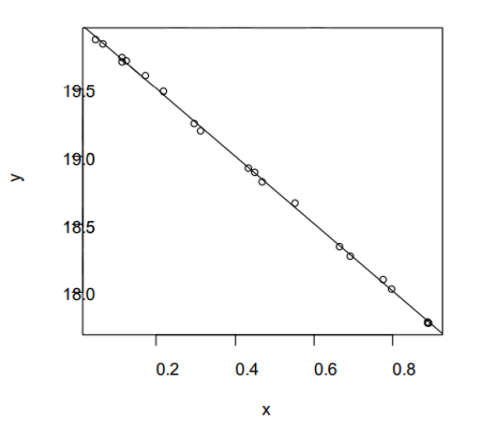
\includegraphics[width=0.5\columnwidth]{figs/3.png}
    \caption{}
    \label{fig:3}
   \end{figure}
    \begin{multicols}{4}
    \begin{enumerate}
        \item -1
        \item 0
        \item 0.05
        \item 1
    \end{enumerate}
    \end{multicols}
    \hfill{$\brak{ GATE\ EY\ 2014}$}
    \bigskip

    \item Death feigning behaviour (i.e., pretending to be dead when attacked) is found in snakes and millipedes. This similarity in behaviour between snakes and millipedes is an example of
    \begin{multicols}{2}
    \begin{enumerate}
        \item convergent evolution
        \item phylogenetic constraint
        \item co-evolution
        \item divergent evolution
    \end{enumerate}
    \end{multicols}
    \hfill{$\brak{ GATE\ EY\ 2014}$}
    \bigskip

    \item To evaluate the relationship between two variables $\brak{e.g.,\ resource\ abundance\ and\ population\ density}$, a linear regression can be used. Here, the statistical null hypothesis which allows us to evaluate whether there is a relationship between these variables is
    \begin{multicols}{2}
    \begin{enumerate}
        \item intercept $=0$
        \item slope $=0$
        \item sample size $=0$
        \item mean $=0$
    \end{enumerate}
    \end{multicols}
    \hfill{$\brak{ GATE\ EY\ 2014}$}
    \bigskip

    \item Which of the following conditions is NOT necessary for evolution by natural selection?
    \begin{multicols}{2}
    \begin{enumerate}
        \item Variation in a trait
        \item Heritability of the trait
        \item Change in the environment
        \item Differential fitness related to the trait
    \end{enumerate}
    \end{multicols}
    \hfill{$\brak{ GATE\ EY\ 2014}$}
    \bigskip
    
    \item $C_{3}$, $C_{4}$ and CAM are the main photosynthetic pathways in plants. The relative abundance of $C_{3}$ plants
    \begin{enumerate}
        \item increases with increasing latitude.
        \item decreases with increasing latitude.
        \item stays the same with increasing latitude.
        \item shows no pattern with increasing latitude.
    \end{enumerate}
    \hfill{$\brak{ GATE\ EY\ 2014}$}
    \bigskip
    
    \item The pyramidal structure of decreasing biomass with increasing trophic level in terrestrial ecosystems is a consequence of:
    \begin{multicols}{2}
    \begin{enumerate}
        \item the second law of thermodynamics
        \item bio-magnification\newline
        \item conservation of energy
        \item increasing competition at higher trophic levels
    \end{enumerate}
    \end{multicols}
    \hfill{$\brak{ GATE\ EY\ 2014}$}
    \bigskip
    
    \item Typical green leaves from plants absorb light of the following colour/s:
    \begin{multicols}{2}
    \begin{enumerate}
        \item green
        \item red and green
        \item all colours
        \item red and blue
    \end{enumerate}
    \end{multicols}
    \hfill{$\brak{ GATE\ EY\ 2014}$}
    \bigskip
    
    \item Christian Bergmann, a $19$th century biologist, observed that related taxa showed increasing body size with increasing latitude. One explanation for this pattern, also called `Bergmann's Rule', is
    \begin{enumerate}
        \item lower body mass in the tropics is a result of lower mass-specific metabolic rates
        \item species at higher latitudes have greater access to resources and, therefore, have larger sizes
        \item greater competition at higher latitudes results in larger organisms
        \item lower surface area to volume ratios in larger animals help conserve heat
    \end{enumerate}
    \hfill{$\brak{ GATE\ EY\ 2014}$}
    \bigskip
    
    \item All else being equal, in a species with two sexes, which of the following is true with regard to mate choice?
    \begin{enumerate}
        \item The sex with the higher number of chromosomes is more likely to be choosy
        \item The sex with the higher number of genes is more likely to be choosy
        \item The sex with the larger gamete is more likely to be choosy
        \item The sex with the smaller gamete is more likely to be choosy
    \end{enumerate}
    \hfill{$\brak{ GATE\ EY\ 2014}$}
    \bigskip
    
    \item Temperate organisms have wider tolerance ranges for temperature than do tropical organisms. If temperatures increase across the globe by $2^{\circ}C$, which of the following is possible?
    \begin{enumerate}
        \item Temperate organisms will be more negatively affected than tropical organisms
        \item Tropical organisms will be more negatively affected than temperate organisms
        \item The effects on tropical and temperate organisms will be the same
        \item This will have no effect on temperate or tropical organisms
    \end{enumerate}
    \hfill{$\brak{ GATE\ EY\ 2014}$}
    \bigskip
    
    \item The length of Henle's loop in the kidneys of rodents is longest in
    \begin{multicols}{2}
    \begin{enumerate}
        \item hot desert habitats
        \item cool temperate habitats
        \item tropical moist habitats
        \item wetland habitats
    \end{enumerate}
    \end{multicols}
    \hfill{$\brak{ GATE\ EY\ 2014}$}
    \bigskip
    
    \item A recent experiment with a fast growing variety of tomato studied the inheritance of two traits dwarfism and flower colour. The experiment successfully demonstrated Mendel's law of segregation and for both traits the expected $3:1$ ratio of dominant to recessive phenotype was observed. However, the experiment failed to demonstrate the law of independent assortment for the two traits. One possible reason for this is
    \begin{multicols}{2}
    \begin{enumerate}
        \item that the two loci are linked
        \item low penetrance of the traits
        \item that the two loci are on different chromosomes
        \item incomplete dominance
    \end{enumerate}
    \end{multicols}
    \hfill{$\brak{ GATE\ EY\ 2014}$}
    \bigskip

    \item Grazing by large herbivores can increase plant diversity by which of the following mechanisms?
    \begin{enumerate}
        \item $\brak{i}$ Accelerating rates of nutrient cycling in the ecosystem
        \item $\brak{ii}$ Reducing abundance of dominant plants and favouring rare plants
        \item $\brak{iii}$ Promoting photo-respiration by increasing ambient $CO_{2}$ concentration
        \item $\brak{iv}$ Decreasing stomatal conductance which promotes biomass production
    \end{enumerate}
    \begin{multicols}{2}
    \begin{enumerate}
        \item Both $\brak{i}$ and $\brak{ii}$
        \item Both $\brak{iii}$ and $\brak{iv}$
        \item Both $\brak{ii}$ and $\brak{iv}$
        \item Both $\brak{i}$ and $\brak{iii}$
    \end{enumerate}
    \end{multicols}
    \hfill{$\brak{ GATE\ EY\ 2014}$}
    \bigskip

    \item The doubling time for a bacterial population is $60$ minutes. Given a density of $35~cells/ml$ in a population in its exponential growth phase and assuming unlimited resources, the number of hours that the population will take to reach a density of $560~cells/ml$ is \rule{3cm}{0.15mm}
    \hfill{$\brak{ GATE\ EY\ 2014}$}
    \bigskip

\end{enumerate}

\noindent \textbf{Q. 26 -- Q. 55} carry two marks each.
\begin{enumerate}
\setcounter{enumi}{25}

    \item Birds that are brood parasites lay eggs in the nests of other birds. This is a successful strategy for the brood parasite when
    \begin{enumerate}
        \item the host bird and the brood parasite bird species are similar in size
        \item the host bird lays fewer eggs than the brood parasite
        \item host birds cannot discriminate between their eggs and those of the parasite
        \item the parasite chicks are much smaller than those of the host bird species
    \end{enumerate}
    \hfill{$\brak{ GATE\ EY\ 2014}$}
    \bigskip

    \item What should be the sound frequency ranges used for acoustic communication between two herds of elephants living far apart in isolated forests, domestic dogs in neighbouring streets, and insect feeding bats catching prey above the tree canopy?
    \begin{enumerate}
        \item High frequency, low frequency and ultrasonic, respectively
        \item High frequency, human hearing range and ultrasonic, respectively
        \item Low frequency, human hearing range and ultrasonic, respectively
        \item Ultrasonic, high frequency and high frequency, respectively
    \end{enumerate}
    \hfill{$\brak{ GATE\ EY\ 2014}$}
    \bigskip

    \item A student grows a bacterial culture in a container starting with a small population size and high resource levels. To estimate population growth, the student puts the container on a weighing machine after air-tight sealing of the container to avoid contamination. Which of the following graphs is the most likely result obtained in the experiment?
    
    \begin{figure}[H]
    \centering
    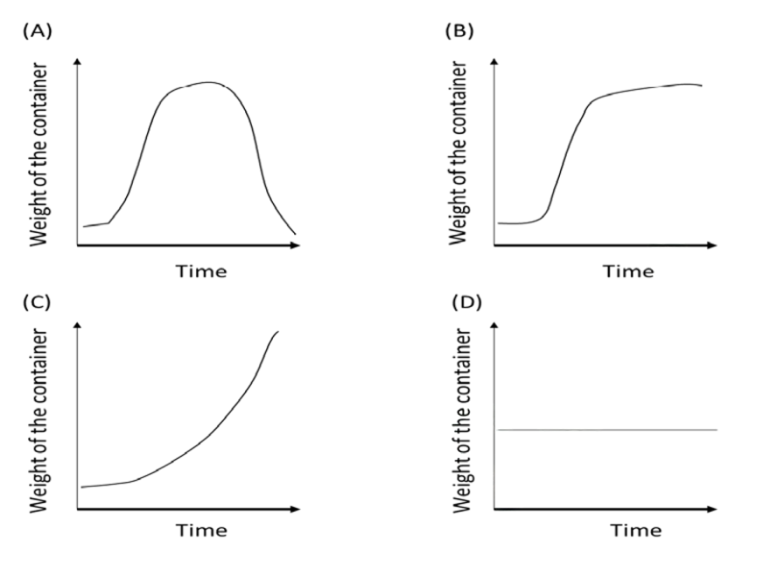
\includegraphics[width=0.7\columnwidth]{figs/4.png}
    \caption{}
    \end{figure}
    \hfill{$\brak{ GATE\ EY\ 2014}$}
    \bigskip

    \item Birds show much variation in sexual size dimorphism $\brak{body\ size\ differences\ between\ males\ and\ females}$, which is hypothesized to be associated with their mating system. Match the two groups below to reflect the expected pattern in mating system and sexual size dimorphism in birds.
    \begin{description}
        \item[Mating system]
        \item[i.] Monogamy $\brak{1\ male\ and\ 1\ female}$
        \item[ii.] Polygyny $\brak{1\ male\ and\ many\ females}$
        \item[iii.] Polyandry $\brak{1\ female\ and\ many\ males}$
        \item[Size dimorphism]
        \item[P.] Males larger than females
        \item[Q.] Females larger than males
        \item[R.] Males and females similar in size
    \end{description}
    \begin{multicols}{2}
    \begin{enumerate}
        \item i -- Q; ii -- P; iii -- R
        \item i -- R; ii -- P; iii -- Q
        \item i -- P; ii -- R; iii -- Q
        \item i -- R; ii -- Q; iii -- P
    \end{enumerate}
    \end{multicols}
    \hfill{$\brak{ GATE\ EY\ 2014}$}
    \bigskip

    \item Consider the following frequency distribution of an ecological variable:
    \begin{figure}[H]
    \centering
    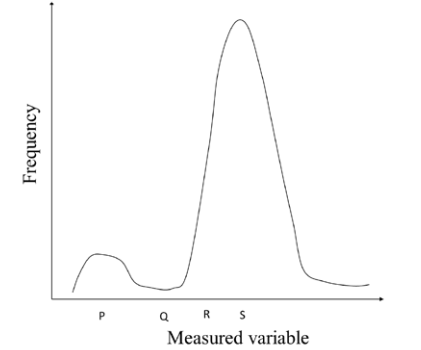
\includegraphics[width=0.7\columnwidth]{figs/5.png}
    \caption{}
    \label{fig:5}
   \end{figure}
    Such a distribution with two peaks is called a bi-modal distribution. Here, the peak with the higher frequency is called the major mode and the one with the lower frequency is called the minor mode. A student has marked four points on the x-axis, i.e., P, Q, R and S. Match the points with the most appropriate statistic: Mean, Median, Major mode, and Minor mode
    \begin{enumerate}
        \item P-Major mode, Q-Mean, R-Median, S-Minor mode
        \item P-Major mode, Q-Median, S-Minor mode
        \item P-Minor mode, R-Mean, S-Major mode
        \item Q-Median, S-Major mode, S-Mean
    \end{enumerate}
    \hfill{$\brak{ GATE\ EY\ 2014}$}
    \bigskip
    
    \item In blackbuck, it has been hypothesized that the reproductive fitness of an individual depends on the group size as given below. Two groups of unrelated individuals,labelled as G$1$ and G$2$,encounter each other. Note that G$2$ is at the optimalgroup size. Individuals from each group can decide whether to stay in their group, or join the other group. Individuals cannot prevent others from leaving or joining any group. Under these circumstances, which of the following is most likely?
    \begin{figure}[H]
    \centering
    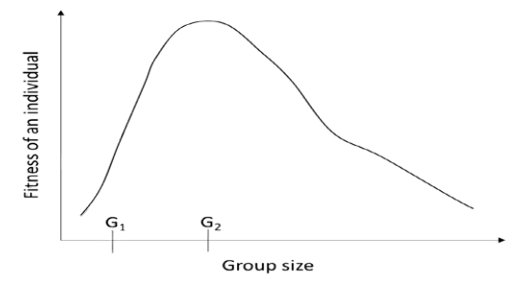
\includegraphics[width=0.7\columnwidth]{figs/6.png}
    \caption{}
    \label{fig:6}
   \end{figure}
   \begin{enumerate}
    
        \item Individuals of G$1$ will choose not to merge with G$2$ because the fitness of individuals of G$2$will decrease
        \item Individuals of G$1$ will choose to merge with G$2$ because it will increase their own fitness
        \item Individuals of G$2$ will choose to merge with G$1$ because it will increase their own fitness
        \item Individuals of G$2$ will choose to merge with G$1$ because the fitness of individuals of G$1$ will increase
    \end{enumerate}
    \hfill{$\brak{ GATE\ EY\ 2014}$}
    \bigskip
    
    \item  In certain cases, a critical group size of organisms is required before a certain action, such as secretion of an enzyme, is taken by individuals of the group. This can be graphically represented as shown below.
    \begin{figure}[H]
    \centering
    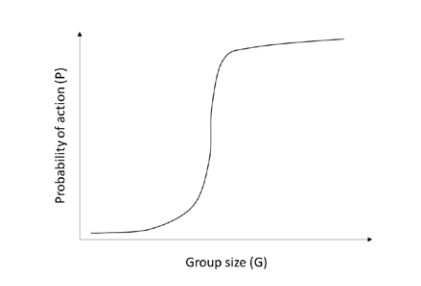
\includegraphics[width=0.5\columnwidth]{figs/7.png}
    \caption{}
    \label{fig:7}
   \end{figure}
    A student conducts experiments and collects data to study this behaviour in her favourite system. Instead of plotting P vs. G, the student plots G $\brak{on\ the\ y-axis}$ vs. P $\brak{on\ the\ x-axis}$. Assuming that her system did indeed exhibit the group behaviour of the type shown above, how will her modified plot look?
   \begin{figure}[H]
    \centering
    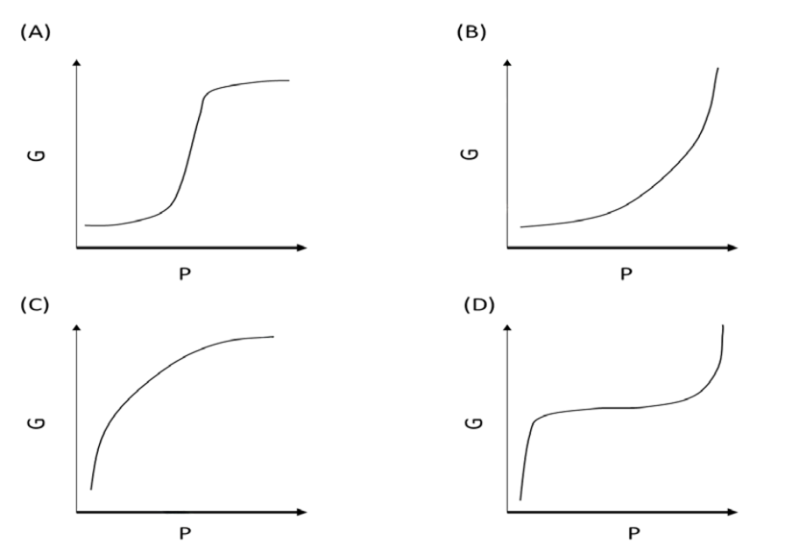
\includegraphics[width=0.7\columnwidth]{figs/8.png}
    \caption{}
    \label{fig:8}
   \end{figure}
    \hfill{$\brak{ GATE\ EY\ 2014}$}
    \bigskip
 \item All adults of a fish species have bright colour patterns in population P and all adults have dull colour patterns in population Q. Colour patterns in this species are determined early in development. Which of the following study designs is best suited to test whether this colour pattern difference has a genetic basis?
    \begin{enumerate}
        \item For each population in its natural habitat, follow $100$ eggs to the adult stage and measure the colour patterns of the adults
        \item Bring $100$ adults of population P and $100$ adults of population Q to the lab, allow them to acclimatize for one day under uniform conditions, and then measure colour patterns of the adults
        \item Bring $100$ adults of population P to the habitat of population Q, allow to acclimatize for one day, and measure colour patterns of the adults; similarly move $100$ adults of population Q to the habitat of population P and measure colour patterns
        \item Bring $100$ eggs of population P and $100$ eggs of population Q to the lab, maintain them at uniform conditions, follow them to the adult stage, and then measure colour patterns of the adults
    \end{enumerate}
    \hfill{$\brak{ GATE\ EY\ 2014}$}
    \bigskip
    
   
      \item The figure below shows how competition among foragers in a resource patch reduces individual foraging rates. According to this figure, the expected foraging rate for a solitary individual is \rule{3cm}{0.15mm}
    \begin{figure}[H]
    \centering
    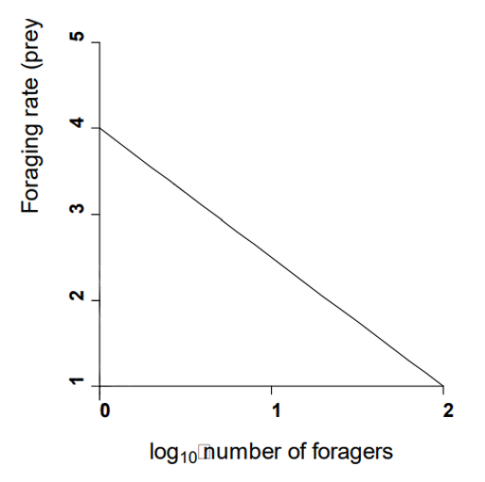
\includegraphics[width=0.6\columnwidth]{figs/9.png}
    \caption{}
    \label{fig:9}
   \end{figure}
    \hfill{$\brak{ GATE\ EY\ 2014}$}
    \bigskip
    
    \item Find the matching triplet
    \begin{figure}[H]
    \centering
    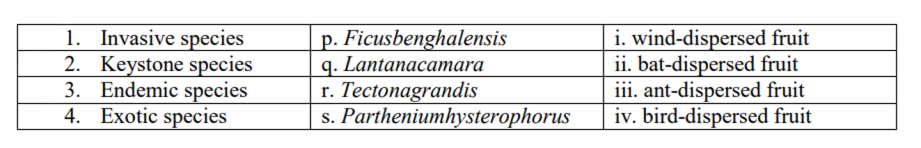
\includegraphics[width=0.8\columnwidth]{figs/10.png}
    \caption{}
    \label{fig:10}
   \end{figure}
    \begin{multicols}{2}
    \begin{enumerate}
        \item 2, r, i
        \item 1, q, iv
        \item 3, s, iii
        \item 4, p, ii
    \end{enumerate}
    \end{multicols}
    \hfill{$\brak{ GATE\ EY\ 2014}$}
    \bigskip
    
\item In birds that pair during the breeding season, it is hypothesized that males need to aggressively guard their mates against mating with intruder males. To test this hypothesis, a scientist presents a male dummy bird to a male bird on his territory just before the female lays her eggs. The dummy is left on the territory. The male was aggressive towards the dummy before the eggs were laid and this aggression declined after egg-laying. Which additional experiment will NOT provide further information to test this hypothesis?
    \begin{enumerate}
        \item Present the dummy to a second set of males in the absence of females
        \item Present the dummy to a second set of males before the eggs are laid and remove the dummy from the territory
        \item Use a live male bird instead of the dummy
        \item Present the dummy to a second set of males only after the eggs are laid
    \end{enumerate}
    \hfill{$\brak{ GATE\ EY\ 2014}$}
    \bigskip

    \item The figure panels below show population growth in two species, when they are grown alone, and also when they are grown together. From the nature of their growth curves, one can infer that the interaction between these species is an example of
    \begin{figure}[H]
    \centering
    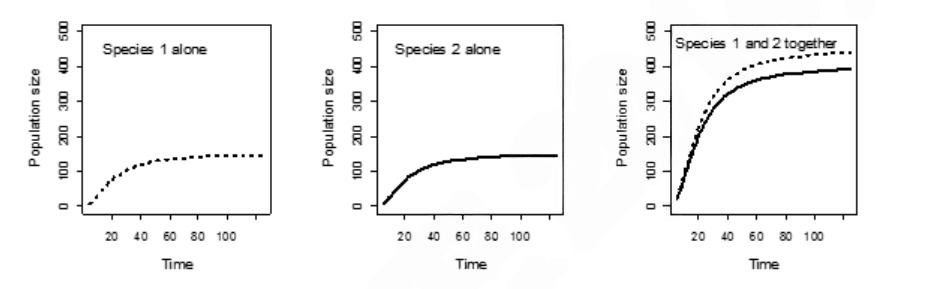
\includegraphics[width=0.8\columnwidth]{figs/11.png}
    \caption{}
    \label{fig:11}
   \end{figure}
    \begin{multicols}{2}
    \begin{enumerate}
        \item mutualism
        \item commensalism
        \item predator-prey
        \item competition
    \end{enumerate}
    \end{multicols}
    \hfill{$\brak{ GATE\ EY\ 2014}$}
    \bigskip

    \item There are two coins in a bowl. Because of differences in the size of the two coins, the probability of picking the bigger coin is $0.6$. The bigger coin is unbiased, whereas the smaller coin has a probability of $0.6$ of yielding heads. A blind-folded student picks a coin from the bowl and tosses the coin. The probability$\brak{expressed\ using\ decimal\ notation,\ not\ as\ a\ fraction\ or\ percentage}$ that the coin yields a head is \rule{3cm}{0.15mm}
    \hfill{$\brak{ GATE\ EY\ 2014}$}
    \bigskip
    
    \item The accompanying figure shows logistic population growth for two species in the same habitat. Which of the following conclusions hold true?
    \begin{figure}[H]
    \centering
    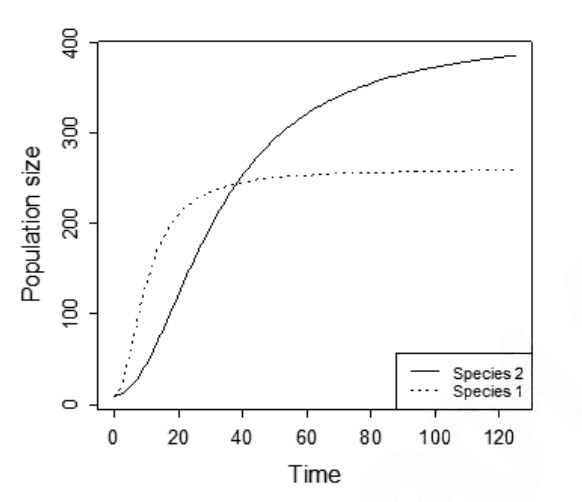
\includegraphics[width=0.7\columnwidth]{figs/12.png}
    \caption{}
    \label{fig:12}
   \end{figure}
    \begin{enumerate}
        \item $\brak{i}$ Species 1 has higher intrinsic growth rate
        \item $\brak{ii}$ Species 2 has higher intrinsic growth rate
        \item $\brak{iii}$ Carrying capacity for Species 1 is higher
        \item $\brak{iv}$ Carrying capacity for Species 2 is higher
    \end{enumerate}
    \begin{multicols}{2}
    \begin{enumerate}
        \item Both $\brak{i}$ and $\brak{iii}$
        \item Both $\brak{i}$ and $\brak{iv}$
        \item Both $\brak{i}$ and $\brak{ii}$
        \item Both $\brak{ii}$ and $\brak{iv}$
    \end{enumerate}
    \end{multicols}
    \hfill{$\brak{ GATE\ EY\ 2014}$}
    \bigskip

    \item Which of these is true with respect to Batesian mimicry?
    \begin{enumerate}
        \item There is a mutualistic relationship between the model and mimic
        \item There is frequency independent selection on the model and the mimic
        \item A mimic exploits the signal of a model
        \item There is positive frequency dependent selection on the mimic
    \end{enumerate}
    \hfill{$\brak{ GATE\ EY\ 2014}$}
    \bigskip

    \item In the phylogeny below, branch lengths are proportional to the percent sequence divergence. The scale below the phylogeny indicates branch length. Assume that the gene used to reconstruct the phylogeny of the species evolves in a clock-like fashion. It is known that the divergence between Species $4$ and Species $5$ happened $2$ million years ago. The time of divergence $\brak{in\ million\ years}$ between Species 3 and Species 1 is \rule{3cm}{0.15mm}
    \begin{figure}[H]
    \centering
    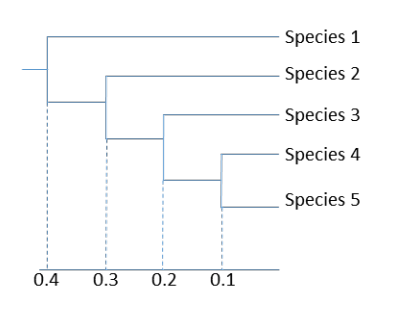
\includegraphics[width=0.7\columnwidth]{figs/13.png}
    \caption{}
    \label{fig:13}
   \end{figure}
    \hfill{$\brak{ GATE\ EY\ 2014}$}
    \bigskip
    
    \item Humans have a preference for high calorie foods. Assume a study has shown that $\brak{i}$ the life expectancy of human beings has reduced from 
    $85$ to $74$ years due to increased consumption of high calorie foods, and $\brak{ii}$ the maximum reproductive age is $70$ years. Given these assumptions, which of the following is most likely to happen in the next $200$ years?
    \begin{enumerate}
        \item Humans will evolve a preference for low calorie foods
        \item Humans will evolve the genes to improve life expectancy when feeding on high calorie foods
        \item Humans will evolve enzymes to extract more energy from low calorie foods
        \item Humans will still have a preference for high calorie foods
    \end{enumerate}
    \hfill{$\brak{ GATE\ EY\ 2014}$}
    \bigskip
    
    \item A recently discovered fossil contains $3.125\%$ of $^{14}$C found in present day organisms. If the half-life of $^{14}$C is $5730$ years, the age of the fossil in years is \rule{3cm}{0.15mm}
    \hfill{$\brak{ GATE\ EY\ 2014}$}
    \bigskip
    
    \item In the hypothetical scenario below, there are four small islands $\brak{P,\ Q,\ R\ and\ S}$ near a very large continent. The distances of the islands from the continent, as well as the sizes of the islands, vary as indicated in the diagram. Assume that dispersal happens only between the continent and the islands, but not among islands. The theory of island biogeography would predict that the number of species in each island will be best represented by which of the following?
    \begin{figure}[H]
    \centering
    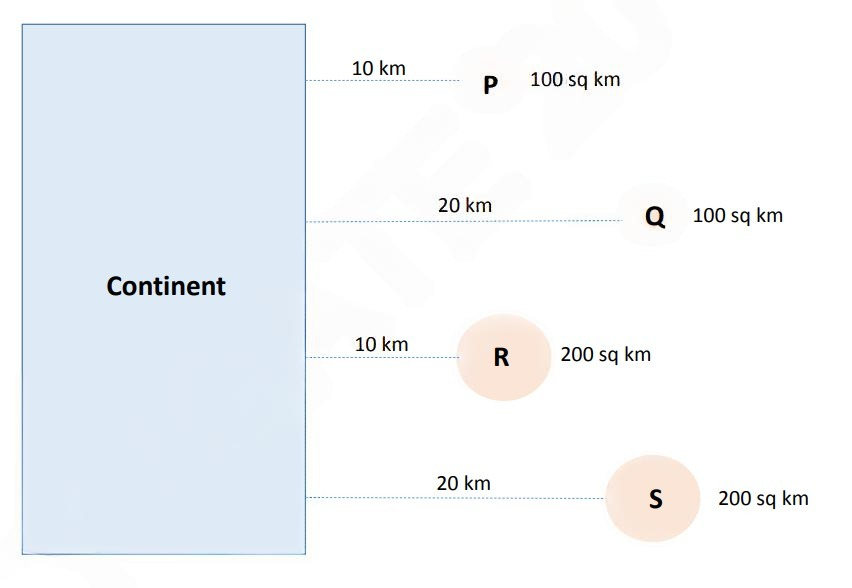
\includegraphics[width=0.7\columnwidth]{figs/14.png}
    \caption{}
    \label{fig:14}
   \end{figure}
    \begin{multicols}{2}
    \begin{enumerate}
        \item $R = S$ and $P = Q$
        \item $R > Q$ and $R > S$
        \item $R > Q$ and $Q > P$
        \item $S > P$ and $Q > S$
    \end{enumerate}
    \end{multicols}
    \hfill{$\brak{ GATE\ EY\ 2014}$}
    \bigskip
    
    \item There are 19500 ants of a species on a small island of area 400 sq m. A student collects 1500 ants in 30 randomly placed pit-fall traps. She marks all of them with blue paint and releases them. Due to unusually low temperatures the following night, the ant population on the island experiences 10\% mortality. The next day the student lays out another series of randomly placed pit-fall traps and collects 1183 ants. Assuming that (i) mortality is not affected by being painted, (ii) probability of falling into a trap is not affected by being painted, and (iii) probability of falling into a trap is not affected by the density of ants on the island, the expected number of ants with blue marks in the sample is \rule{3cm}{0.15mm}
    \hfill{$\brak{ GATE\ EY\ 2014}$}
    \bigskip
    
    \item A student wants to test the effect of latitude and longitude on seed size in a plant species. He has the resources to lay a maximum of 9 plots. Which plot design is most appropriate for this question?
    \begin{figure}[H]
    \centering
    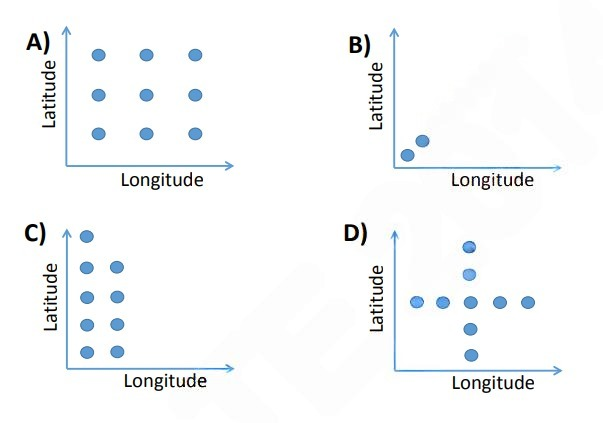
\includegraphics[width=0.7\columnwidth]{figs/15.png}
    \caption{}
    \label{fig:15}
   \end{figure}
    \hfill{$\brak{ GATE\ EY\ 2014}$}
    \bigskip
    
    \item In an experiment, cows were allowed to graze in closed pastures either with wild deer or without wild deer. This experiment was done in the rainy and dry seasons. The results for weight gain in the cows (mean and 95\% confidence interval) are shown in the figure below. Based on these results which of the following statements is true?
    \begin{figure}[H]
    \centering
    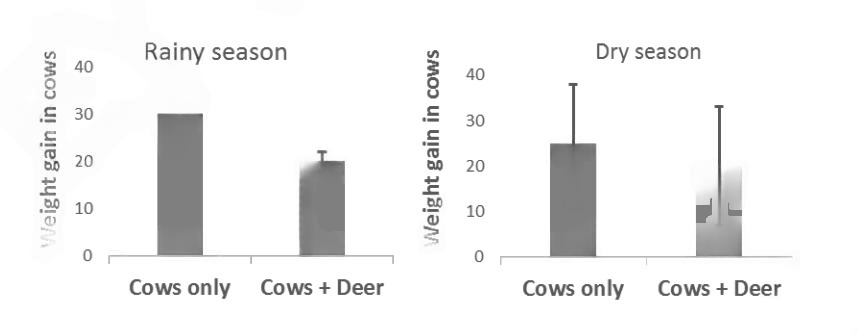
\includegraphics[width=0.7\columnwidth]{figs/16.png}
    \caption{}
    \label{fig:16}
   \end{figure}
    \begin{enumerate}
        \item The presence of wild deer does not affect weight gain in cows
        \item The effect of wild deer on weight gain in cows changes with season
        \item The presence of wild deer has an inhibitory effect on weight gain in cows in both seasons
        \item Cows and wild deer have a mutualistic relationship in the dry season
    \end{enumerate}
    \hfill{$\brak{ GATE\ EY\ 2014}$}
    \bigskip

    \item The figure below shows how reproductive fitness varies with tail length in a bird species. Given this pattern, what kind of selection is most likely to act on tail length in this population?
    \begin{figure}[H]
    \centering
    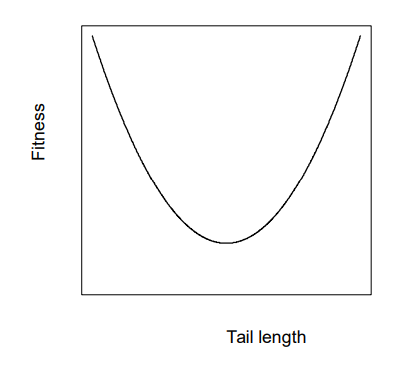
\includegraphics[width=0.7\columnwidth]{figs/17.png}
    \caption{}
    \label{fig:17}
   \end{figure}
    \begin{multicols}{4}
    \begin{enumerate}
        \item Relaxed
        \item Directional
        \item Disruptive
        \item Stabilizing
    \end{enumerate}
    \end{multicols}
    \hfill{$\brak{ GATE\ EY\ 2014}$}
    \bigskip

    \item A study monitored insect abundance and drought stress in trees for a period of 10 years in a tropical dry deciduous forest. This study found a strong, statistically significant, negative relationship between insect abundance and drought stress in trees. Based on these results, what can be inferred about the causal relationship between insect abundance and drought stress in trees?
    \begin{enumerate}
        \item Increased insect abundance causes increased drought stress in trees
        \item Increased drought stress in trees causes increase in insect abundance
        \item Decreased drought stress in trees causes increase in insect abundance
        \item No direct causal relationship can be inferred from these data
    \end{enumerate}
    \hfill{$\brak{ GATE\ EY\ 2014}$}
    \bigskip

    \item Assume that a piece of bamboo is a hollow cylinder of negligible wall thickness. The numerical value (in cm) of the ratio of the volume to surface area of such a bamboo, measuring 6 cm in diameter, is \rule{3cm}{0.15mm}
    \hfill{$\brak{ GATE\ EY\ 2014}$}
    \bigskip

    \item Simpson's index of species diversity is given by
    $$D = \frac{1}{\sum_{i=1}^{n} p_i^2}$$
    where $p_i$ is the proportion of species i in the total sample of individuals and n is the total number of species. For the species and their abundances given below, the numerical value of Simpson's index is \rule{3cm}{0.15mm}
    \begin{figure}[H]
    \centering
    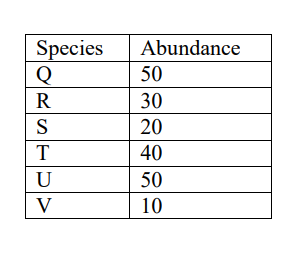
\includegraphics[width=0.7\columnwidth]{figs/18.png}
    \caption{}
    \label{fig:18}
   \end{figure}
    \hfill{$\brak{ GATE\ EY\ 2014}$}
    \bigskip

    \item Primary succession refers to the sequence of changes in plant communities at a newly formed habitat. Species establishing first at the newly formed habitat (pioneer species) show characteristics that are different from those in species that establish later in the community. Which of the following represents the predicted characteristics of pioneer species?
    \begin{enumerate}
        \item Large dispersal distance, high fecundity, low competitive ability, short lifespan
        \item Short dispersal distance, high fecundity, high competitive ability, short lifespan
        \item Large dispersal distance, high fecundity, high competitive ability, long lifespan
        \item Short dispersal distance, low fecundity, high competitive ability, long lifespan
    \end{enumerate}
    \hfill{$\brak{ GATE\ EY\ 2014}$}
    \bigskip
\newpage
    \item Consider the two phylogenies. Which of the following statements is true?
    \begin{figure}[H]
    \centering
    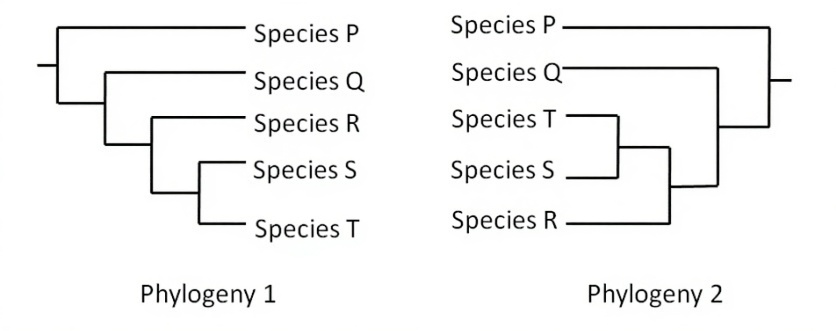
\includegraphics[width=0.7\columnwidth]{figs/19.png}
    \caption{}
    \label{fig:19}
   \end{figure}
   \begin{enumerate}
        \item The two phylogenies are the same
        \item The relationship between P and Q is the same in both phylogenies, whereas the relationships among R, S and T differ between the two phylogenies
        \item Q and R are more closely related to each other in phylogeny 1 than in phylogeny 2
        \item R diverged from S and T earlier in phylogeny 1 than in phylogeny 2
    \end{enumerate}
    \hfill{$\brak{ GATE\ EY\ 2014}$}
    \item Species P and Species Q are respectively self-pollinated and cross-pollinated plants that are closely related. Their flowers are visited by bees. Correctly identify which sets of traits are characteristic of Species P relative to the traits of Species Q.
    \begin{enumerate}
        \item larger flowers, scented flowers, and fewer pollen grains per flower
        \item larger flowers, unscented flowers, and more pollen grains per flower
        \item smaller flowers, unscented flowers, and fewer pollen grains per flower
        \item smaller flowers, scented flowers, and more pollen grains per flowers
    \end{enumerate}
    \hfill{$\brak{ GATE\ EY\ 2014}$}
   \\
    \item The Venn Diagram below shows numbers of species in three forest types. Which of the following statements is true?
    \begin{figure}[H]
    \centering
    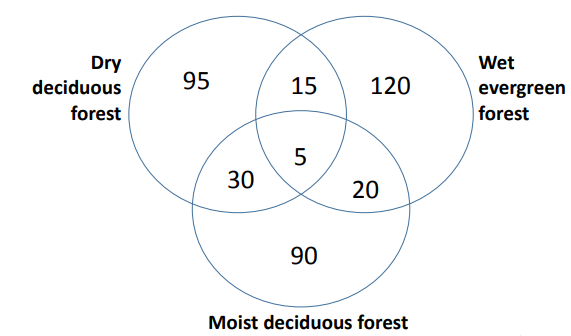
\includegraphics[width=0.4\columnwidth]{figs/20.png}
    \caption{}
    \label{fig:20}
   \end{figure}
    \begin{enumerate}
        \item Overlap of species between dry deciduous and moist deciduous $>$ overlap between moist deciduous and wet evergreen
        \item Overlap of species between wet evergreen and dry deciduous $>$ overlap between wet evergreen and moist deciduous
        \item Total species in dry deciduous $>$ moist deciduous
        \item Total species in moist deciduous $>$ wet evergreen
    \end{enumerate}
    \hfill{$\brak{ GATE\ EY\ 2014}$}
    \bigskip
    
\end{enumerate}
\begin{center}
\Large
\textbf{END OF THE QUESTION PAPER}
\end{center}
\end{document}
